\chapter{Background}

\section{The Maritime Connectivity Platform}
The Maritime Connectivity Platform (MCP), which is formally known as the Maritime Cloud is a platform, developed by EfficienSea2 \cite{efficienSea2}, which is led by the Danish Maritime Consortium. MCP is a communication framework, that is to ensure efficient, reliable and secure communication, and exchange of information in the maritime sector.
The goal of the platform is to connect maritime stakeholders with maritime information services.
\begin{figure}
	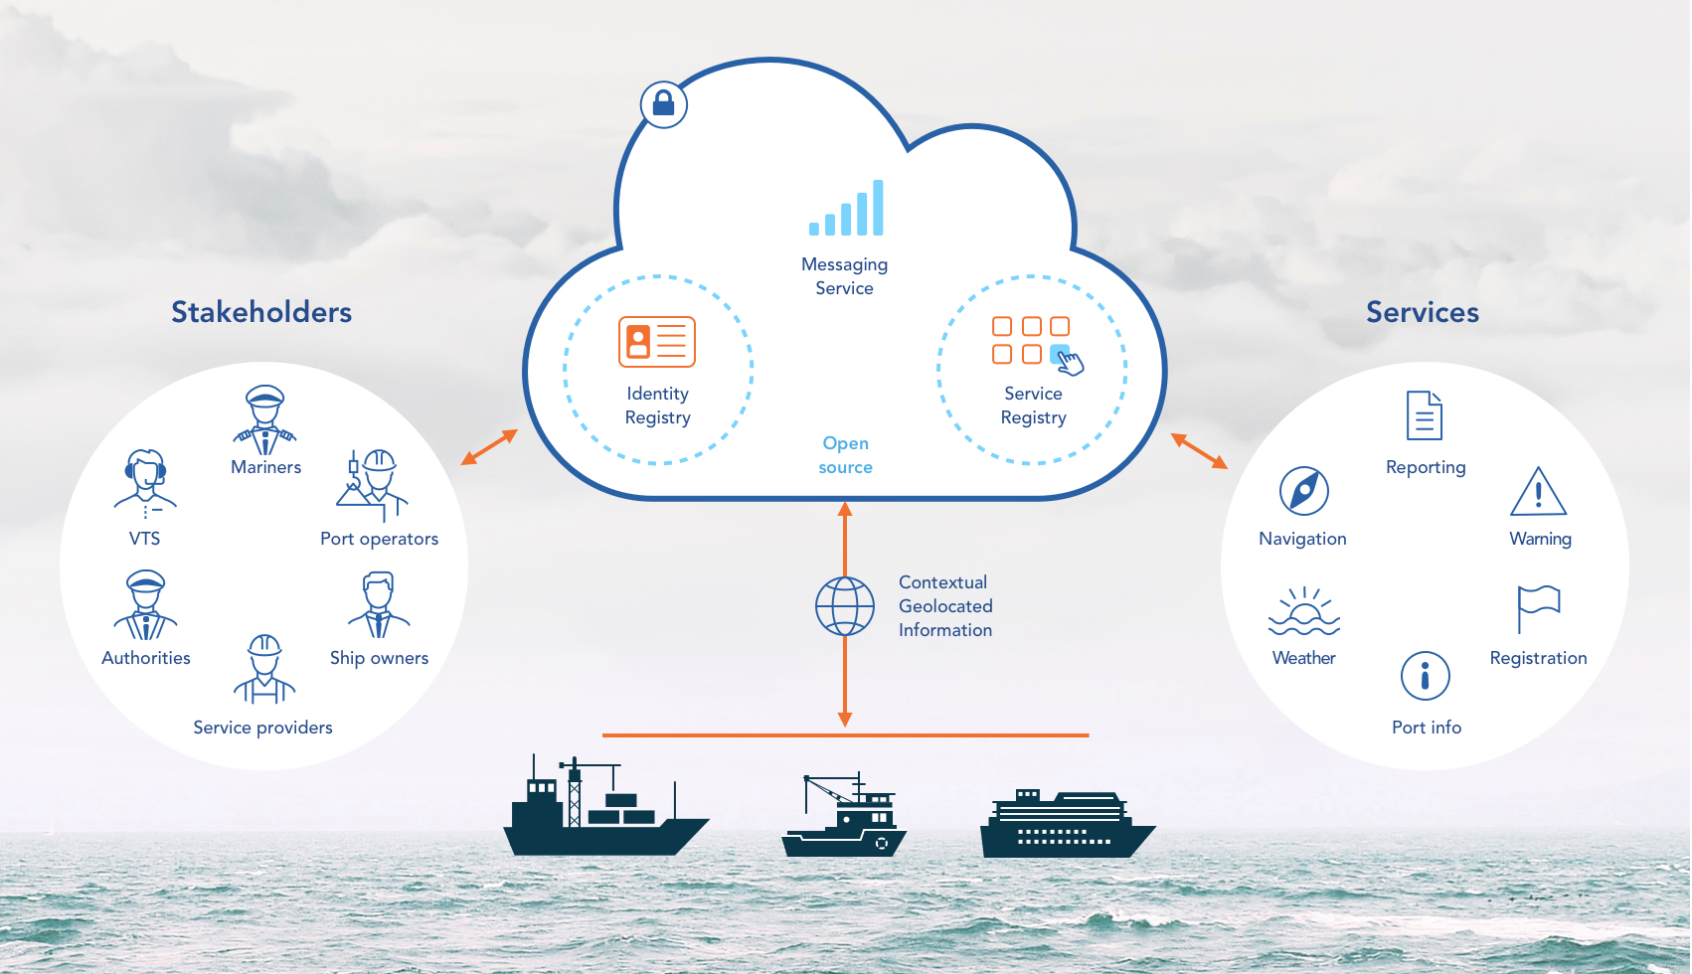
\includegraphics[width=1\textwidth]{figures/MCPStructure}
	\caption{Diagram, describing the structure of MCP. \cite{efficienSea2}}
	\label{fig:MCPStruct}
\end{figure}\noindent
A high-level diagram, describing the structure of the MCP can be seen in Figure \ref{fig:MCPStruct}. Here it is shown that maritime stakeholders are connected with the maritime services through the Identity Registry, the Service Registry and the Messaging Service.

\subsection{Identity Registry}
Here the relevant information regarding maritime stakeholders are stored. This information needs to be authorized and stored at a safe location in order for the security of the MCP to be sufficient. The Identity Registry on the MCP is equivalent to the Central Person Registry of a country. The Identity Registry is vital to the MCP in it ensures the solution's authenticity, integrity, and confidentiality. Maritime stakeholders are, through the Identity Registry provided with a single login to all Maritime Services.\cite{efficienSea2}
\subsection{Service Registry}
The Service Registry acts to Maritime Services as the Identity Registry acts to the Maritime Stakeholders. Here all Maritime Services are registered and stored. The Service Registry holds both commercial and non-commercial, as well as authorized and non-authorized services, either free of charge or for a fee. The Service Registry is comparable with the App Store or Google Play in that it distributes services of all kinds to registered users.\cite{efficienSea2}
\subsection{Messaging Service}
\tit{"An information broker that intelligently exchanges information between communication systems connected to the platform, taking into account the current geographical position and communication links available to the recipient."}\cite{efficienSea2}

\section{Monadic Parsing}

Text parsing is a functionality, supported in virtually every programming language.

\section{Property-Based Testing}

Property based testing, also known as Automation Testing, is the principle of testing properties of code, rather than instances, as is done in manual unit testing. Unit tests are fast and easy to set up and execute, however, in most instances they only provide coverage to a certain degree. Depending on the complexity of the given program, most programmers can come up with tests, covering most of the given program, however many edge-cases are unintuitive and would require extensive testing to determine manually.

Property-based testing solves this problem by setting up test cases that take into account mathematical models, describing the desired behavior of the code. Once such a test case has been created, semi-random execution instances can be run to the point of literal exhaustion, and thus a relatively small program can test for thousands of occurrences at once.

An example of this can be seen in Listing \ref{lst:pbtEx}, that describe a snippet of Haskell quicksort code. A property of quicksort is that a list, sorted once is equivalent to a list, sorted twice, which is what the function \ttt{prop\_idempotent} validates.

\begin{lstlisting}[caption={Example of Property-Based Testing. \cite{realWorldHaskell11}}, captionpos={below}, label={lst:pbtEx}]
import Test.QuickCheck
import Data.List

qsort :: Ord a => [a] -> [a]
qsort []     = []
qsort (x:xs) = qsort lhs ++ [x] ++ qsort rhs
    where lhs = filter  (< x) xs
          rhs = filter (>= x) xs

prop_idempotent xs = qsort (qsort xs) == qsort xs
\end{lstlisting}


\section{Model-Based Testing}

The principle of Model-based testing is to check behavior of software against predictions made by a model. Behavior can be described in a variety of manners, including data flow, control flow, dependencies, decision trees/cycles, and state transition machines. Model-based testing is good at describing the behavior of a system, when it reacts to a specific action, which is determined by another specific model. Using this technique, the behavior of a system can easily be determined and validated. Currently there are two main types of model-based testing-techniques:

\begin{itemize}
	\item \tbf{Serial model building- and testing:}\\
	This way of implementing model-based testing involves predefined models, upon which a number of tests are executed. Creating the model ahead of execution allows the tester to implement an additional layer of complexity to the created models. Depending on the amount of models, this is, however, a significantly slower process than the alternative, in that each model requires a similar amount of time to construct. Figure \ref{fig:serialMBT} provides a high-level diagram, describing this principle, using arbitrary units of measurement along it's $x$- and $y$-axis.\\
	\begin{figure}
		\centering
		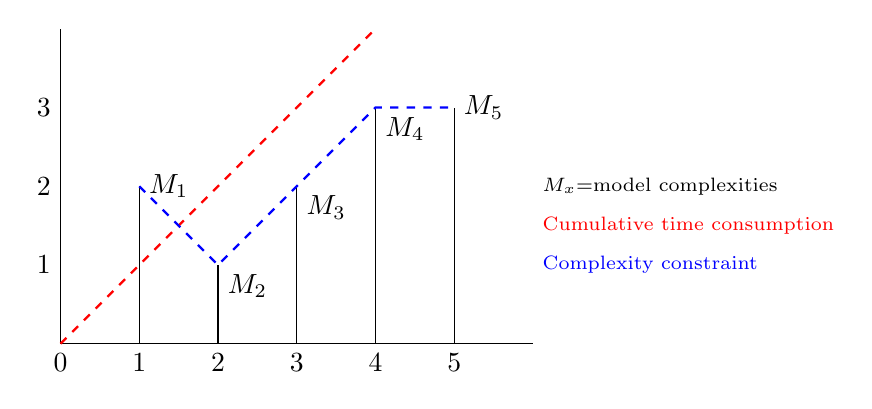
\begin{tikzpicture}
			% horizontal and vertical axis
			\draw	(0,0) -- (6,0)
					(0,0) -- (0,4);

			% horizontal and vertical labels
			\draw	(0,0)	node[anchor=north]	{0}
					(1,0)	node[anchor=north]	{1}
					(2,0)	node[anchor=north]	{2}
					(3,0)	node[anchor=north]	{3}
					(4,0)	node[anchor=north]	{4}
					(5,0)	node[anchor=north]	{5}

					(0,1)	node[anchor=east]	{1}
					(0,2)	node[anchor=east]	{2}
					(0,3)	node[anchor=east]	{3};
			
			% legend
			\draw	(6,2)	node[anchor=west] {\scriptsize $M_x$=model complexities}
					(6,1.5)	node[anchor=west] {\scriptsize\color{red} {Cumulative time consumption}}
					(6,1)	node[anchor=west] {\scriptsize\color{blue} Complexity constraint};
			
			% models
			\draw	(1,0) -- (1,2) node[anchor=west]		{$M_1$}
					(2,0) -- (2,1) node[anchor=north west]	{$M_2$}
					(3,0) -- (3,2) node[anchor=north west]	{$M_3$}
					(4,0) -- (4,3) node[anchor=north west]	{$M_4$}
					(5,0) -- (5,3) node[anchor=west]		{$M_5$};

			% cumulative time consumption
			\draw[dashed, red, thick]	(0,0) -- (4,4);
			% complexity constraint
			\draw[dashed, blue, thick]	(1,2) -- (2,1) -- (3,2) -- (4,3) -- (5,3);
		\end{tikzpicture}
		\caption{Time consumption and complexity restraint of serial model building and testing.}
		\label{fig:serialMBT}
	\end{figure}
	Figure \ref{fig:serialMBT} shows the time consumption increasing for every model built, while the model complexity is directly matching the requirement, set by each specific model.
	\item \tbf{Sequential model building- and testing:}\\
	This way of implementing model-based testing involves on-the-fly model creation- and testing. Here a program is designed to take in arguments, describing different model behaviors, upon the basis of which the program tests the models immediately after they are generated. Compared with the implementation described above, this technique scales to a much better degree, as the program will only need to be written once in order to create a virtually infinite amount of models. The created models are, however, constrained to the lowest common complexity level, shared across all of the generated models. Figure \ref{fig:sequenceMBT} provides a high-level diagram, describing this principle, using arbitrary units of measurement along it's $x$- and $y$-axis.
	\begin{figure}
		\centering
		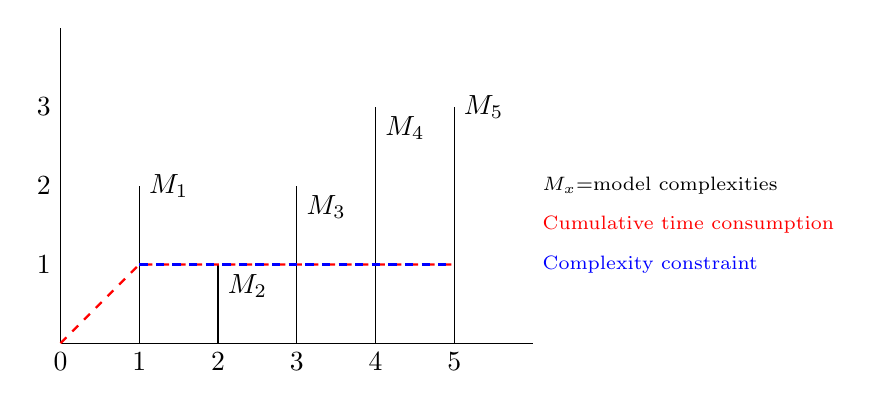
\begin{tikzpicture}
			% horizontal and vertical axis
			\draw	(0,0)	--	(6,0)
					(0,0)	--	(0,4);

			% horizontal and vertical labels
			\draw	(0,0)	node[anchor=north]	{0}
					(1,0)	node[anchor=north]	{1}
					(2,0)	node[anchor=north]	{2}
					(3,0)	node[anchor=north]	{3}
					(4,0)	node[anchor=north]	{4}
					(5,0)	node[anchor=north]	{5}

					(0,1)	node[anchor=east]	{1}
					(0,2)	node[anchor=east]	{2}
					(0,3)	node[anchor=east]	{3};
			
			% legend
			\draw	(6,2)	node[anchor=west] {\scriptsize $M_x$=model complexities}
					(6,1.5)	node[anchor=west] {\scriptsize\color{red} {Cumulative time consumption}}
					(6,1)	node[anchor=west] {\scriptsize\color{blue} Complexity constraint};
			
			% models
			\draw	(1,0)	--	(1,2)	node[anchor=west]		{$M_1$}
					(2,0)	--	(2,1)	node[anchor=north west]	{$M_2$}
					(3,0)	--	(3,2)	node[anchor=north west]	{$M_3$}
					(4,0)	--	(4,3)	node[anchor=north west]	{$M_4$}
					(5,0)	--	(5,3)	node[anchor=west]		{$M_5$};

			% cumulative time consumption
			\draw[dashed, red, thick]	(0,0)	--	(1,1)	--	(5,1);
			% complexity constraint
			\draw[dashed, blue, thick]	(1,1)	--	(5,1);
		\end{tikzpicture}
		\caption{Time consumption and complexity restraint of sequential model building and testing.}
		\label{fig:sequenceMBT}
	\end{figure}
	Figure \ref{fig:sequenceMBT} shows that the time consumption halts to a stop when one model is built with the drawback that the model complexity constraint is set to the lowest common model.
\end{itemize}


\subsection{Finite State Machines (FSM)}
A finite state machine is, as the name suggests, a mathematical machine, consisting of a collection of states. An arbitrary FSM has a start state along with a collection of states that are accessed through various status- and/or input-combinations. An example of this can be seen in Figure \ref{fig:fsmEx} as well as Table \ref{tab:fsmEx}. These describe the control flow of a turnstile, which allows for one pass through, after which it prompts for a coin before allowing another pass through.

\begin{figure}
	\centering
	\begin{tikzpicture}[->,>=stealth', node distance=3.5 cm, thick]
		\tikzstyle{every state}=[draw=black,rectangle,rounded corners]

		\node[state, initial]	(A)	[]				{Locked};
		\node[state]			(B)	[right of=A]	{Unlocked};

		\path	(A)	edge	[bend	left,	above]	node	{Insert Coin}	(B)
					edge	[loop	above,	above]	node	{Pass Through}			(A)
				(B)	edge	[bend	left,	below]	node	{Pass Through}			(A)
					edge	[loop	above,	above]	node	{Insert Coin}	(B);
	\end{tikzpicture}
	\caption{Example of a finite state machine, describing a turnstile. Furthermore, this figure describes Table \ref{tab:fsmEx}.}
	\label{fig:fsmEx}
\end{figure}

\begin{table}[h!]
	\centering
	\begin{tabular}{l|l|l|l}\toprule
		State		& action		& Next State	& Output \\ \midrule
		Locked		& Insert Coin	& Unlocked		& Unlocks turnstile, allowing passage. \\
		Locked		& Push			& Locked		& Blocks passage. \\
		Unlocked	& Insert Coin	& Unlocked		& Returns coin. \\
		Unlocked	& Push			& Locked		& Allows passage, locks. \\ \bottomrule
	\end{tabular}
	\caption{Example of a finite state machine, describing a turnstile. Furthermore, this table describes Figure \ref{fig:fsmEx}.}
	\label{tab:fsmEx}
\end{table}

\subsection{State Charts}
